% IEEE DG 2027 (2027 IEEE 4th International Student Conference on Digital Generation)
% Layout follows the conference Word template (A4; margins: top 1.9 cm, bottom 4.3 cm,
% left/right 2.0 cm; title 20 pt, author names 11 pt, body 10 pt Times).
% Compile: pdflatex main && bibtex main && pdflatex main && pdflatex main
\documentclass[conference,a4paper]{IEEEtran}
\IEEEoverridecommandlockouts
\usepackage[a4paper,top=1.9cm,bottom=4.3cm,left=2cm,right=2cm,columnsep=0.5cm]{geometry}
\usepackage[utf8]{inputenc}
\usepackage[T1]{fontenc}
\usepackage{amsmath,amssymb}
\usepackage{graphicx}
\usepackage{booktabs}
\usepackage{url}
\usepackage{cite}
\usepackage{eso-pic}
\usepackage[hidelinks]{hyperref}

% Conference line in the top-left corner of the first page (as in the template)
\AddToShipoutPictureFG*{%
  \AtPageUpperLeft{\put(\LenToUnit{2cm},\LenToUnit{-1.25cm}){%
    \parbox[t]{12cm}{\fontsize{7}{8}\selectfont 2027 IEEE 4th International Student Conference on Digital Generation (DG)\\
    24--26 February, 2027, Astana, Kazakhstan}}}}

\begin{document}

\title{\fontsize{20}{24}\selectfont Confidence-Aware Graph Neural Networks for Social Bot Detection: Message-Passing Reweighting and Similarity-Graph Construction}

\author{
\IEEEauthorblockN{\fontsize{11}{13}\selectfont Kanalbay Kassymkhan}
\IEEEauthorblockA{\textit{School of Software Engineering}\\
\textit{Astana IT University}\\
Astana, Kazakhstan\\
255479@astanait.edu.kz}
\and
\IEEEauthorblockN{\fontsize{11}{13}\selectfont La Lira L'vovna}
\IEEEauthorblockA{\textit{L.N. Gumilyov Eurasian National University}\\
Astana, Kazakhstan\\
Lira.La@astanait.edu.kz}
}

\maketitle

\begin{abstract}
Graph neural networks are increasingly used to detect social bots, but a standard graph convolutional network weights neighbor messages by node degree only. We study confidence-aware message passing, in which every neighbor is reweighted by the model's own predictive confidence from the previous epoch, and three extensions: an adaptive variant with a learnable exponent applied on top of the baseline normalization, agreement-based edge weights, and pseudo-label self-training. Using a labeled Twitter dataset of 5000 accounts, repeated cross-validation, paired significance tests and ablations, we compare these models with feature-only, GCN, GraphSAGE and GAT baselines and study how the similarity graph between accounts is built. Graph construction is the decisive design choice. On a nearest-neighbor graph of profile descriptions every convolutional model is worse than a feature-only network, whereas on a graph of account metadata every graph model outperforms it. GraphSAGE on the metadata graph reaches an F1 score of 0.840 and an area under the ROC curve of 0.921, which is 3.2 F1 points above the feature-only model and 9.9 points above the original pipeline. With only 250 to 500 labeled accounts, GraphSAGE with confidence-based self-training is the best model. Confidence reweighting itself is correct and inexpensive but does not outperform the baselines, and its learned exponents shrink below one.
\end{abstract}

\begin{IEEEkeywords}
social bot detection, graph neural networks, message passing, confidence weighting, self-training, graph construction
\end{IEEEkeywords}

\section{Introduction}
Social bots inflate follower counts, manufacture trends and spread disinformation at scale \cite{cresci2020decade}. Because bots operate in coordinated clusters and reuse templated text, relational structure carries signal that a per-account classifier cannot see, which has motivated graph neural networks (GNNs) for bot detection \cite{alhosseini2019detect,feng2021botrgcn,feng2022rgt}. A graph convolutional network (GCN) \cite{kipf2017gcn}, however, weights each neighbor by degree only: an ambiguous account near the decision boundary contributes as much as one classified with near-certainty, so noisy signal can leak across the class boundary.

Our earlier work \cite{kassymkhan2026conf} proposed a Confidence-Aware GCN (Conf-GCN) that scales each neighbor's message by the model's own softmax confidence and reported, on a single split, a 3.0-point precision gain at a 7.6-point recall cost. This paper tests that claim rigorously and extends the method. We ask: (RQ1) is the gain real, and is it caused by the confidence signal? (RQ2) do adaptive extensions, namely a learnable exponent on top of the baseline normalization, agreement-based edge weights and self-training, help? (RQ3) how much does the construction of the similarity graph matter? (RQ4) what changes when only a few hundred accounts are labeled?

Our contributions are: (1) an adaptive family of confidence-aware layers (AC-GCN, AC-SAGE) that reduces exactly to GCN or GraphSAGE when the exponent is zero; (2) an evaluation with 25 runs per model, paired Wilcoxon tests with Holm correction and ablations that separate confidence from its confounders; (3) a graph-construction study showing that a metadata graph turns GNNs from worse than a feature-only model into the best detectors, improving F1 by 9.9 points over the original pipeline; (4) a label-scarce study in which confidence-based self-training gives the best detector; and (5) public code and per-run results\footnote{\url{https://github.com/solodancer235-star/confidence-aware-gcn-bot-detection}}.

\section{Related Work}
Feature-based detectors such as Botometer combine many profile and activity features in supervised ensembles \cite{davis2016botornot}; they degrade as bots imitate humans and generalize poorly across datasets \cite{yang2020scalable,lee2021discriminative}. Graph-based detectors propagate information along social or similarity edges with GCN, GraphSAGE \cite{hamilton2017sage} or relational models \cite{feng2021botrgcn,feng2022rgt}, evaluated on benchmarks such as TwiBot-20 \cite{feng2021twibot20}. Graph attention networks (GAT) learn edge weights from features \cite{velickovic2018gat}, and the benefit of message passing depends strongly on homophily \cite{zhu2020beyond}. ConfGCN \cite{vashishth2019confgcn} learns per-node label-distribution confidences with extra parameters; we instead use the classifier's own softmax output with no extra parameters. Confident predictions are also used as pseudo-labels in self-training \cite{lee2013pseudo,li2018deeper}, while softmax confidence is known to be imperfectly calibrated \cite{guo2017calibration}. For tabular data without explicit links, a $k$-nearest-neighbor ($k$-NN) graph over embeddings \cite{reimers2019sbert} is a common substitute \cite{zhu2003semi}.

\section{Method}

\subsection{Confidence-Aware GCN}
Let $c_j=\max_k \mathrm{softmax}(z_j)_k$ be the confidence of node $j$ computed from its logits $z_j$ in the previous epoch ($c_j\in[0.5,1]$ for two classes). Conf-GCN replaces the degree normalization of GCN by
\begin{equation}
h_i^{(l+1)}=\sigma\Big(\sum_{j\in\mathcal{N}(i)}\frac{c_j}{\sum_{k\in\mathcal{N}(i)}c_k}\,W^{(l)}h_j^{(l)}\Big).
\label{eq:conf}
\end{equation}
Confidence is initialized to one, recomputed after every epoch by a no-gradient evaluation pass, and never receives gradients; it uses no labels. The layer adds no parameters, and for equal confidences it reduces to mean aggregation without a self-loop, which is \emph{not} the symmetric normalization of GCN. Since $c_j\in[0.5,1]$, two neighbors of a node differ in weight by at most a factor of two.

\subsection{Adaptive Confidence-Aware GNNs}
To isolate the confidence signal, AC-GCN keeps the GCN weights $a_{ji}=1/\sqrt{\hat d_i\hat d_j}$ over $\mathcal{N}(i)\cup\{i\}$ and only redistributes their mass:
\begin{equation}
w_{ji}^{(l)}=a_{ji}\,c_j^{\alpha_l}\,\frac{\sum_k a_{ki}}{\sum_k a_{ki}\,c_k^{\alpha_l}},\qquad \alpha_l=\mathrm{softplus}(\rho_l)\ge 0 .
\label{eq:acgcn}
\end{equation}
With $\alpha_l=0$ or constant confidence the layer equals GCN exactly; the three learnable exponents (one per layer, initialized at one) let the model amplify or ignore confidence and remove the factor-two bound. AC-SAGE applies the same idea to the neighbor mean of GraphSAGE, $h_i'=W_rh_i+W_n\sum_j \tilde w_{ji}h_j$. The \emph{agreement} variant replaces $c_j^{\alpha_l}$ by $(\sum_k p_{jk}p_{ik})^{\alpha_l}$, the probability that both endpoints share a class, which can switch edges off entirely. In \emph{self-training} (+ST), after 20 warm-up epochs every unlabeled node with confidence of at least 0.9 receives its predicted class as a pseudo-label with loss weight 0.5.

\subsection{Similarity-Graph Construction}
The dataset has no follow graph, so we compare three label-free symmetrized cosine $k$-NN graphs ($k=10$): over description embeddings (\emph{description graph}, edge homophily 0.617), over the ten z-scored metadata fields (\emph{metadata graph}, 0.777), and over both (\emph{feature graph}, 0.756).

\section{Experimental Setup}
\textbf{Data.} We use the Twitter human/bot dataset \cite{gutierrez2021twitter} (labels from Botometer and manual verification) in a cleaned English-only redistribution \cite{botani2024} with 29\,407 accounts, and draw a balanced stratified subsample of 5000 accounts. Node features (394 dimensions) are a 384-dimensional Sentence-BERT embedding of the description \cite{reimers2019sbert}, six log-transformed numeric fields standardized on training nodes, and four binary flags.

\textbf{Models.} A feature-only multilayer perceptron (MLP), GCN, GraphSAGE (mean), GAT and our models, all with three layers, hidden size 64 and dropout 0.5, implemented in PyTorch Geometric \cite{fey2019pyg}. Learning rate and weight decay (and GAT heads) are selected by validation F1; extensions reuse the setting of their base model; training runs for 100 epochs.

\textbf{Protocol.} Stratified 5-fold cross-validation repeated over 5 seeds (25 runs per model, 60/20/20 train/validation/test). We report precision, recall and F1 for the bot class and the area under the ROC curve (AUROC), and compare models with paired Wilcoxon signed-rank tests with Holm correction \cite{demsar2006statistical,holm1979simple}. The label-scarce study trains on 100, 250 or 500 labeled accounts over 10 random splits.

\section{Results}

\subsection{Conf-GCN Under Repeated Cross-Validation (RQ1)}
Table~\ref{tab:main} shows that the single-split precision gain does not replicate: Conf-GCN and GCN have the same precision (0.732 vs.\ 0.731, $p=0.83$), Conf-GCN loses 0.9 F1 points ($p=0.004$) and 2.5 AUROC points, and the feature-only MLP is the best model. The run-to-run standard deviation of F1 (about 0.02) is as large as the earlier single-split differences.

\begin{table}[htbp]
\caption{Description graph, 25 runs (mean $\pm$ std). $p$: paired Wilcoxon of F1 vs.\ Conf-GCN, Holm-corrected.}
\label{tab:main}
\centering
\footnotesize
\setlength{\tabcolsep}{3pt}
\begin{tabular}{@{}lccccc@{}}
\toprule
Model & Prec. & Rec. & F1 & AUROC & $p$\\
\midrule
MLP (no graph) & 0.805 & 0.809 & 0.807$\pm$0.010 & 0.890 & $<$0.001\\
GCN & 0.731 & 0.752 & 0.740$\pm$0.016 & 0.819 & 0.004\\
GraphSAGE & 0.805 & 0.801 & 0.803$\pm$0.014 & 0.887 & $<$0.001\\
GAT & 0.744 & 0.726 & 0.734$\pm$0.020 & 0.819 & 0.230\\
Conf-GCN & 0.732 & 0.732 & 0.731$\pm$0.019 & 0.794 & ---\\
\bottomrule
\end{tabular}
\end{table}

\begin{table}[htbp]
\caption{Ablations of Conf-GCN, description graph (25 runs). $p$: F1 vs.\ full model, Holm-corrected.}
\label{tab:abl}
\centering
\footnotesize
\setlength{\tabcolsep}{3pt}
\begin{tabular}{@{}lccc@{}}
\toprule
Variant & F1 & AUROC & $p$\\
\midrule
Conf-GCN (full, $\alpha=1$) & 0.731 & 0.794 & ---\\
Uniform confidence ($c\equiv1$) & 0.736 & 0.795 & 0.026\\
Shuffled confidence & 0.735 & 0.795 & 0.104\\
Inverted weighting & 0.733 & 0.797 & 0.668\\
$\alpha=2$ / $\alpha=4$ & 0.728 / 0.727 & 0.793 / 0.788 & 0.668\\
Uniform confidence + self-loop & 0.742 & 0.817 & $<$0.001\\
GCN (reference) & 0.740 & 0.819 & 0.015\\
\bottomrule
\end{tabular}
\end{table}

The ablations in Table~\ref{tab:abl} locate the cause. Discarding confidence (uniform), shuffling it across nodes or even inverting it to favor the \emph{least} confident neighbors leaves the result unchanged, so the behavior of Conf-GCN comes from its normalization. Adding a self-loop to the uniform layer recovers GCN-level performance (F1 0.742, AUROC 0.817): the AUROC gap was caused by the node's own features being diluted. At matched recall, a GCN with a tuned threshold is 0.9 points \emph{more} precise than Conf-GCN ($p<0.001$), so the precision-oriented operating point is not a property of the method. On the real data the confidence weights deviate from uniform aggregation by only 6.5\% on average (largest-to-smallest weight in a neighborhood: median 1.45).

\subsection{Graph Construction (RQ3)}
Table~\ref{tab:graph} shows that changing only the graph reverses the conclusion about GNNs. On the metadata graph every GNN beats the MLP ($p<2\times10^{-5}$ for each), and GraphSAGE becomes the best detector of the study with F1 0.840 and AUROC 0.921, which is 3.2 F1 points above the MLP and 9.9 F1 points above the original description-graph GCN ($p<10^{-6}$). Precision and recall improve together (0.842 and 0.838 vs.\ 0.731 and 0.752). GraphSAGE benefits most because its root transformation keeps a node's own features next to the aggregated neighborhood. The density of the graph matters far less: for $k\in\{5,10,20\}$ GCN on the description graph varies only between 0.732 and 0.740 F1.

\begin{table}[htbp]
\caption{F1 (AUROC) for three $k$-NN graphs, $k=10$, 25 runs. Edge homophily: 0.617 / 0.777 / 0.756.}
\label{tab:graph}
\centering
\footnotesize
\setlength{\tabcolsep}{3pt}
\begin{tabular}{@{}lccc@{}}
\toprule
Model & Description & Metadata & Feature\\
\midrule
GCN & 0.740 (0.819) & 0.826 (0.915) & 0.820 (0.905)\\
GraphSAGE & 0.803 (0.887) & \textbf{0.840 (0.921)} & 0.825 (0.906)\\
GAT & 0.734 (0.819) & 0.823 (0.912) & 0.814 (0.898)\\
Conf-GCN & 0.731 (0.794) & 0.824 (0.912) & 0.818 (0.901)\\
\midrule
MLP (no graph) & \multicolumn{3}{c}{0.807 (0.890)}\\
\bottomrule
\end{tabular}
\end{table}

\subsection{Adaptive Extensions (RQ2)}
Applying confidence on top of GCN's own normalization removes the weakness of the original layer: on the description graph AC-GCN reaches F1 0.737 and AUROC 0.819, the same as GCN and 2.5 AUROC points above Conf-GCN. On the feature graph AC-GCN (0.818), the agreement-weighted GCN (0.818) and AC-SAGE (0.822) stay within 0.4 F1 points of GCN (0.820) and GraphSAGE (0.825), and none is significantly better (Holm-corrected $p\ge0.16$). On the metadata graph AC-SAGE is slightly worse than GraphSAGE (0.835 vs.\ 0.840). The learned exponents explain why: starting from one, they converge to about 0.6--0.7 for AC-GCN and 0.76--0.78 for AC-SAGE, that is, given the freedom to amplify confidence, the models reduce it. Confidence is only moderately predictive of whether a neighbor is correct (AUROC 0.66 on the description graph), so amplifying it would also amplify errors.

\subsection{Few Labeled Accounts (RQ4)}
Labels are expensive in moderation. Fig.~\ref{fig:labels} shows that the graph matters most when labels are few. GraphSAGE with confidence-based self-training is the best model with 100, 250 and 500 labels (F1 0.764, 0.781 and 0.795 vs.\ 0.744, 0.761 and 0.773 for the MLP; $p=0.002$ at 250 and 500 labels, $p=0.06$ at 100). Self-training adds 0.6 F1 points to GraphSAGE at 250 labels ($p=0.014$) and about 1 point to GCN. Here confidence is useful, but as a filter for pseudo-labels rather than as a weight inside message passing.

\begin{figure}[htbp]
\centering
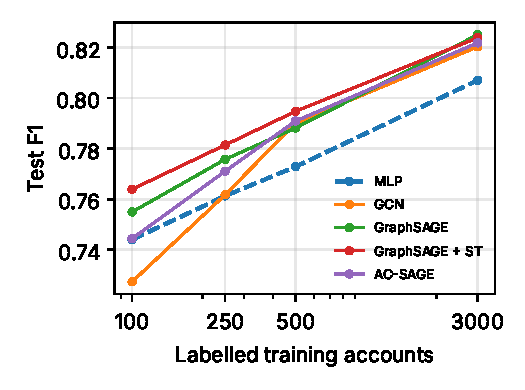
\includegraphics[width=0.95\columnwidth]{figures/fig_labels.pdf}
\caption{Test F1 versus the number of labeled training accounts (feature graph; 10 splits for 100--500 labels, 25 runs for 3000).}
\label{fig:labels}
\end{figure}

\section{Discussion}
The study yields a simple recipe for bot detection on tabular account data: build the similarity graph from account metadata and use an aggregator that keeps a node's own features; with few labels, add confidence-based self-training. Confidence reweighting inside message passing is cheap and, in its adaptive form, as accurate as its baselines, but in the binary case its weights stay close to uniform, whereas graph construction changes which accounts are neighbors at all. Limitations: the graphs are similarity graphs built from the same features used for classification, labels partly come from Botometer (a metadata-based detector), and we used a 5000-account English-only subsample; real follow or mention graphs may behave differently. Runs share data across folds, so $p$-values are indicative.

\section{Conclusion}
We evaluated confidence-aware message passing for social bot detection with repeated cross-validation, paired tests and ablations. The earlier single-split precision gain of Conf-GCN was sampling noise, and neither learnable exponents nor agreement weights improve on GCN or GraphSAGE. The decisive factor is the graph: a metadata $k$-NN graph turns every GNN into a better detector than a feature-only model, and GraphSAGE on it reaches F1 0.840 and AUROC 0.921, 9.9 F1 points above the original pipeline; with only a few hundred labels, confidence-based self-training on this graph gives the best results. Future work will evaluate the recipe on graphs with explicit follow and mention edges such as TwiBot-20 \cite{feng2021twibot20} and learn the graph jointly with the classifier.

\section*{Acknowledgment}
The authors thank the School of Software Engineering at Astana IT University for its support.

\bibliographystyle{IEEEtran}
\bibliography{refs}

\end{document}
